\begin{figure}[h!]
    \centering % Center the figure
    
    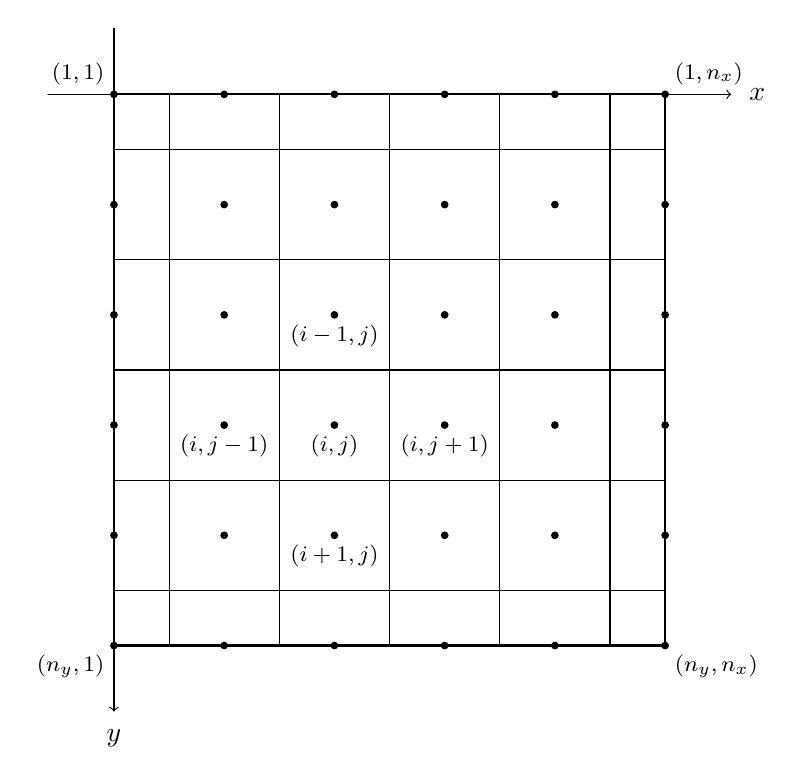
\begin{tikzpicture}[scale=1.4, line cap=round, line join=round]
        % parameters
        \def\nx{6}   % number of centers along x   (i = 1..nx)
        \def\ny{6}   % number of centers along y   (j = 1..ny)
        \def\dx{1} % interior-cell edge in x     (distance between centers)
        \def\dy{1} % interior-cell edge in y

        % domain frame: centers (1,1) at (0,0), (nx,ny) at ((nx-1)dx,(ny-1)dy)
        \pgfmathsetmacro{\xmin}{0}
        \pgfmathsetmacro{\ymin}{0}
        \pgfmathsetmacro{\xmax}{(\nx-1)*\dx}
        \pgfmathsetmacro{\ymax}{(\ny-1)*\dy}

        % external rectangle
        \draw[thick] (\xmin,\ymin) rectangle (\xmax,\ymax);

        % internal faces are mid-planes between adjacent centers
        % vertical faces
        \foreach \k in {1,...,\numexpr\nx-1\relax}{
            \pgfmathsetmacro{\x}{(\k-0.5)*\dx}
            \draw (\x,\ymin) -- (\x,\ymax);
        }
        
        % horizontal faces
        \foreach \l in {1,...,\numexpr\ny-1\relax}{
            \pgfmathsetmacro{\y}{(\l-0.5)*\dy}
            \draw (\xmin,\y) -- (\xmax,\y);
        }

        % centers: first layer lies on the frame, corners included
        \foreach \i in {1,...,\nx}{
            \foreach \j in {1,...,\ny}{
                \pgfmathsetmacro{\xc}{(\i-1)*\dx}
                \pgfmathsetmacro{\yc}{(\j-1)*\dy}
                \fill (\xc,\yc) circle (1-2pt);
            }
        }

        % axes
        \draw[->] (\xmin-0.6,\ymax) -- (\xmax+0.6,\ymax) node[right=3pt] {$x$};
        \draw[->] (0,\ymax+0.6) -- (0,\ymin-0.6) node[below=3pt] {$y$};

        % key labels
        \node[below left]   at (\xmin,\ymin) {\footnotesize $(n_y,1)$};
        \node[below right]  at (\xmax,\ymin) {\footnotesize $(n_y,n_x)$};
        \node[above left]   at (\xmin,\ymax) {\footnotesize $(1,1)$};
        \node[above right]  at (\xmax,\ymax) {\footnotesize $(1,n_x)$};

        % example generic (i,j)
        \pgfmathsetmacro{\xg}{(\nx>3 ? 2*\dx : \dx)}
        \pgfmathsetmacro{\yg}{(\ny>3 ? 2*\dy : \dy)}
        \node[below] at (\xg,\yg) {\footnotesize $(i,j)$};

        \pgfmathsetmacro{\xg}{(\nx>3 ? \dx : \dx)}
        \node[below] at (\xg,\yg) {\footnotesize $(i,j-1)$};

        \pgfmathsetmacro{\xg}{(\nx>3 ? 3*\dx : \dx)}
        \node[below] at (\xg,\yg) {\footnotesize $(i,j+1)$};

        \pgfmathsetmacro{\xg}{(\nx>3 ? 2*\dx : \dx)}
        \pgfmathsetmacro{\yg}{(\ny>3 ? \dy : \dy)}
        \node[below] at (\xg,\yg) {\footnotesize $(i+1,j)$};

        \pgfmathsetmacro{\yg}{(\ny>3 ? 3*\dy : \dy)}
        \node[below] at (\xg,\yg) {\footnotesize $(i-1,j)$};
    \end{tikzpicture}
    
    \caption{Indexing convention.}
    \label{indexing_sketch_split}
\end{figure}